%% This is an example first chapter.  You should put chapter/appendix that you
%% write into a separate file, and add a line \include{yourfilename} to
%% main.tex, where `yourfilename.tex' is the name of the chapter/appendix file.
%% You can process specific files by typing their names in at the 
%% \files=
%% prompt when you run the file main.tex through LaTeX.

\chapter{Dummy chapter}

\begin{quote}
\textit{In this chapter, I describe my introduction. Lorem ipsum dolor sit amet, consectetur adipiscing elit. Aenean quis dolor bibendum, lobortis mauris a, sollicitudin lacus.}
\end{quote}

\newthought{Lorem ipsum dolor sit amet}, consectetur adipiscing elit. Aenean quis dolor bibendum, lobortis mauris a, sollicitudin lacus. Vivamus sollicitudin orci sed convallis faucibus. Morbi tempor augue vel nunc mollis euismod. Fusce varius fermentum dui, vel ultrices massa fermentum a. \marginnote{Check it out, here's a margin note.}  Pellentesque ac ipsum et libero cursus posuere. Aliquam tincidunt sapien ut ultrices dignissim. Cras tortor leo, pulvinar sagittis lacus et, convallis consectetur quam. Suspendisse potenti. Etiam convallis velit felis, eu rutrum ligula dictum sit amet.

Sed nec suscipit ex. Ut quis urna interdum tortor sollicitudin iaculis. Aliquam purus est, venenatis ac blandit quis, semper quis felis. Integer arcu augue, accumsan at vulputate sed, tristique eu libero.\autocite{Aghaeepour2013} Vivamus ut scelerisque massa. Pellentesque commodo arcu mollis dolor venenatis eleifend. Nulla sit amet rutrum nulla. Nullam leo ante, dapibus vel ipsum quis, bibendum condimentum ligula. Sed faucibus fermentum condimentum. Morbi eu ligula id lacus mattis pharetra. Phasellus auctor est sit amet sapien facilisis molestie vel in ipsum. Etiam malesuada vitae eros sed lacinia.\autocite{Rolph2015} Suspendisse eget iaculis odio, a molestie ex. Mauris ultrices et dolor nec dictum.\autocite{Rolph2015}

Vivamus elementum vehicula orci id mollis.\autocite{Aghaeepour2013,Gelman2006} Duis auctor sapien vel pretium bibendum. Nam aliquam, felis at efficitur pretium, justo libero cursus nisi, sit amet molestie metus massa nec sapien. Donec efficitur porttitor arcu et tempus. Phasellus pretium, diam id suscipit ultrices, lectus odio suscipit risus, at fermentum leo massa vitae eros. Donec elit orci, faucibus et aliquet quis, interdum eget lorem. Nulla a tincidunt odio, vitae commodo metus. Pellentesque bibendum cursus.\autocite{Rolph2015}

\section{Methods}

Aliquam purus est, venenatis ac blandit quis, semper quis felis. Integer arcu augue, accumsan at vulputate sed, tristique eu libero. Vivamus ut scelerisque massa. Pellentesque commodo arcu mollis dolor venenatis eleifend. Nulla sit amet rutrum nulla. Nullam leo ante, dapibus vel ipsum quis, bibendum condimentum ligula. Sed faucibus fermentum condimentum. Morbi eu ligula id lacus mattis pharetra. Phasellus auctor est sit amet sapien facilisis molestie vel in ipsum. Etiam malesuada vitae eros sed lacinia. Suspendisse eget iaculis odio, a molestie ex. Mauris ultrices et dolor nec dictum.

\begin{figure}[htb]
  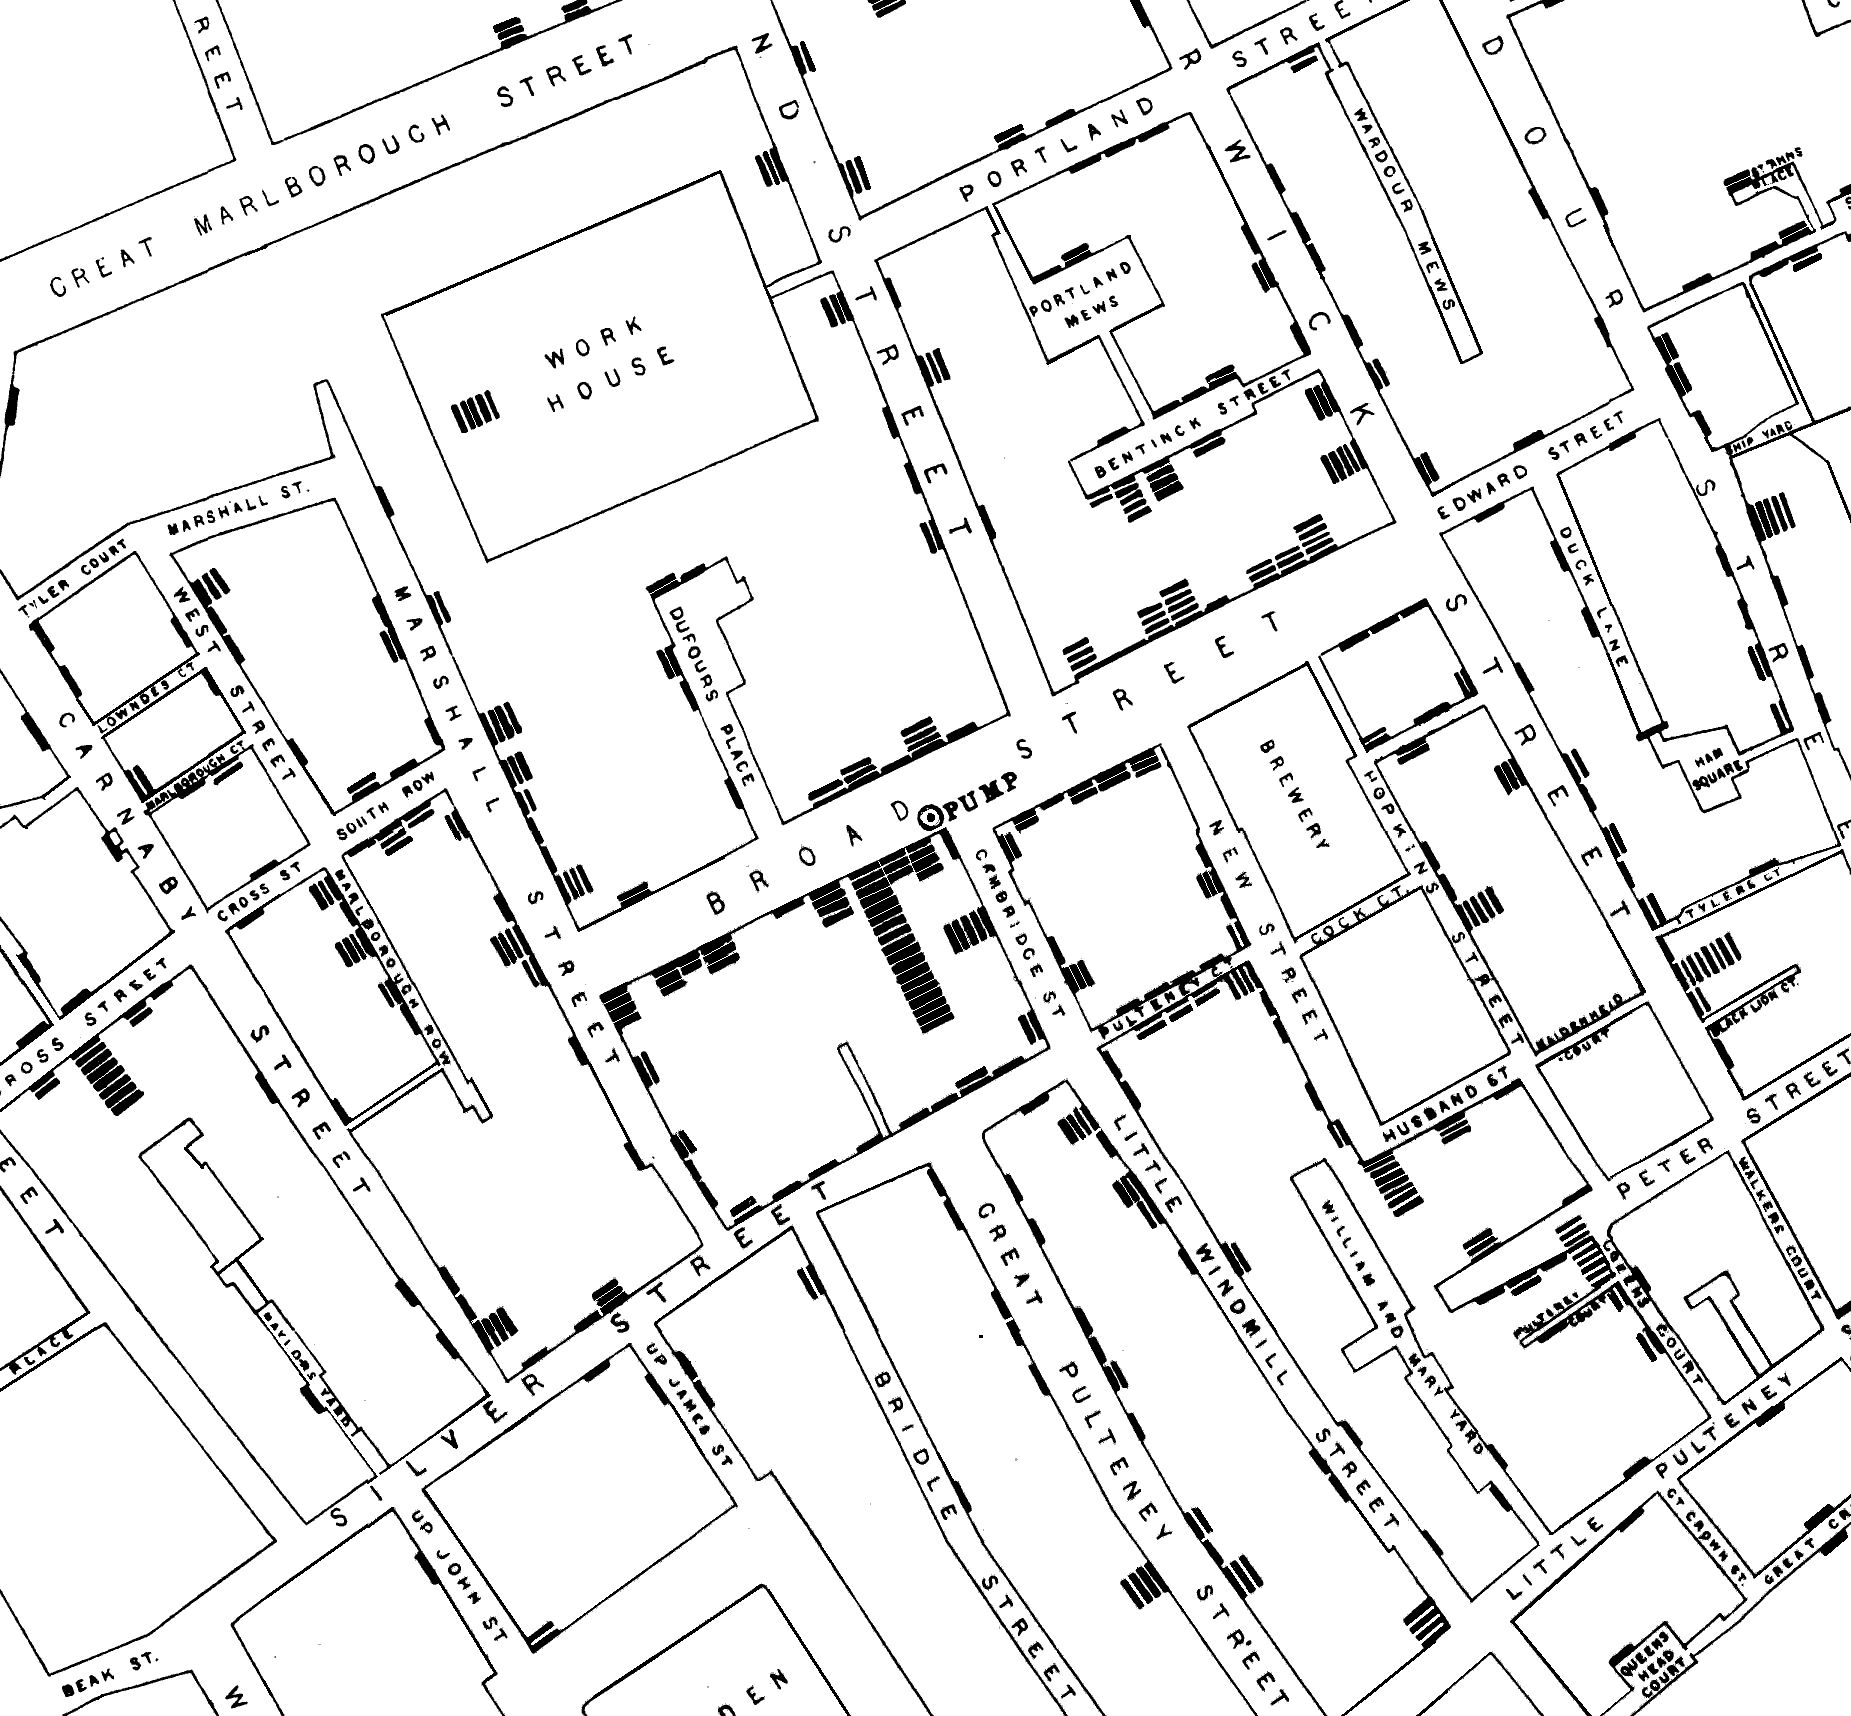
\includegraphics[width=\textwidth]{chap1/snow_map}               
  \caption{John Snow's map does not reveal the ending of Game of Thrones.}
  \label{fig:spin}
\end{figure}

Phasellus eu nunc eget ante hendrerit porta. Etiam dignissim, mauris vitae luctus sollicitudin, metus purus iaculis tortor, eu lobortis arcu neque vitae ante. Donec egestas nec sem id vulputate. Ut efficitur non massa eget tempor. Nullam rhoncus odio sed dui fringilla semper. Nullam luctus odio felis, ac rutrum mauris maximus sodales. Phasellus non gravida nulla. Aenean congue sapien vitae facilisis luctus. Cum sociis natoque penatibus et magnis dis parturient montes, nascetur ridiculus mus. In laoreet ultrices tellus sed tincidunt. Aenean tempus, dui vel fermentum laoreet, sapien sapien facilisis turpis, vel volutpat sapien libero at mi. Maecenas eleifend libero in enim finibus, eu hendrerit ipsum ornare. Nulla placerat massa eget sapien tincidunt, non venenatis libero accumsan. Nunc ex lectus, rutrum sed varius sed, consectetur vel nisl. Aliquam eu eros vel metus sodales fermentum. Sed quis ultrices nisl, vel semper nibh (Table \ref{tab:sample_table}).

\begin{table}[ht]
  \centering
  \begin{tabular}{l l l l l}
    \toprule
    Column A & Column B & Column C & Column D & Column E \\
    \midrule
    A & B & C & D & E \\
    1 & 2 & 3 & 4 & 5 \\
    10 & 20 & 30 & 40 & 50 \\
    \bottomrule
  \end{tabular}
  \caption{A meaningless table}
  \label{tab:sample_table}
\end{table}

Donec elit orci, faucibus et aliquet quis, interdum eget lorem. Nulla a tincidunt odio, vitae commodo metus.

\subsection{Jiggering the pokery}

\newthought{Sed nec suscipit ex.} Ut quis urna interdum tortor sollicitudin iaculis. Aliquam purus est, venenatis ac blandit quis, semper quis felis. Integer arcu augue, accumsan at vulputate sed, tristique eu libero. Vivamus ut scelerisque massa. Pellentesque commodo arcu mollis dolor venenatis eleifend. Nulla sit amet rutrum nulla. Nullam leo ante, dapibus vel ipsum quis, bibendum condimentum ligula. Sed faucibus fermentum condimentum. Morbi eu ligula id lacus mattis pharetra. Phasellus auctor est sit amet sapien facilisis molestie vel in ipsum. Etiam malesuada vitae eros sed lacinia. Suspendisse eget iaculis odio, a molestie ex. Mauris ultrices et dolor nec dictum.\autocite{Rolph2015,Couderc2015}

Duis auctor sapien vel pretium bibendum. Nam aliquam, felis at efficitur pretium, justo libero cursus nisi, sit amet molestie metus massa nec sapien. Donec efficitur porttitor arcu et tempus. Phasellus pretium, diam id suscipit ultrices, lectus odio suscipit risus, at fermentum leo massa vitae eros. Donec elit orci, faucibus et aliquet quis, interdum eget lorem. Nulla a tincidunt odio, vitae commodo metus. Pellentesque bibendum cursus (Figure \ref{fig:spin_margin}).

Ut quis urna interdum tortor sollicitudin iaculis. Aliquam purus est, venenatis ac blandit quis, semper quis felis. Integer arcu augue, accumsan at vulputate sed, tristique eu libero. Vivamus ut scelerisque massa. Pellentesque commodo arcu mollis dolor venenatis eleifend. Nulla sit amet rutrum nulla. Nullam leo ante, dapibus vel ipsum quis, bibendum condimentum ligula.

\begin{marginfigure}
  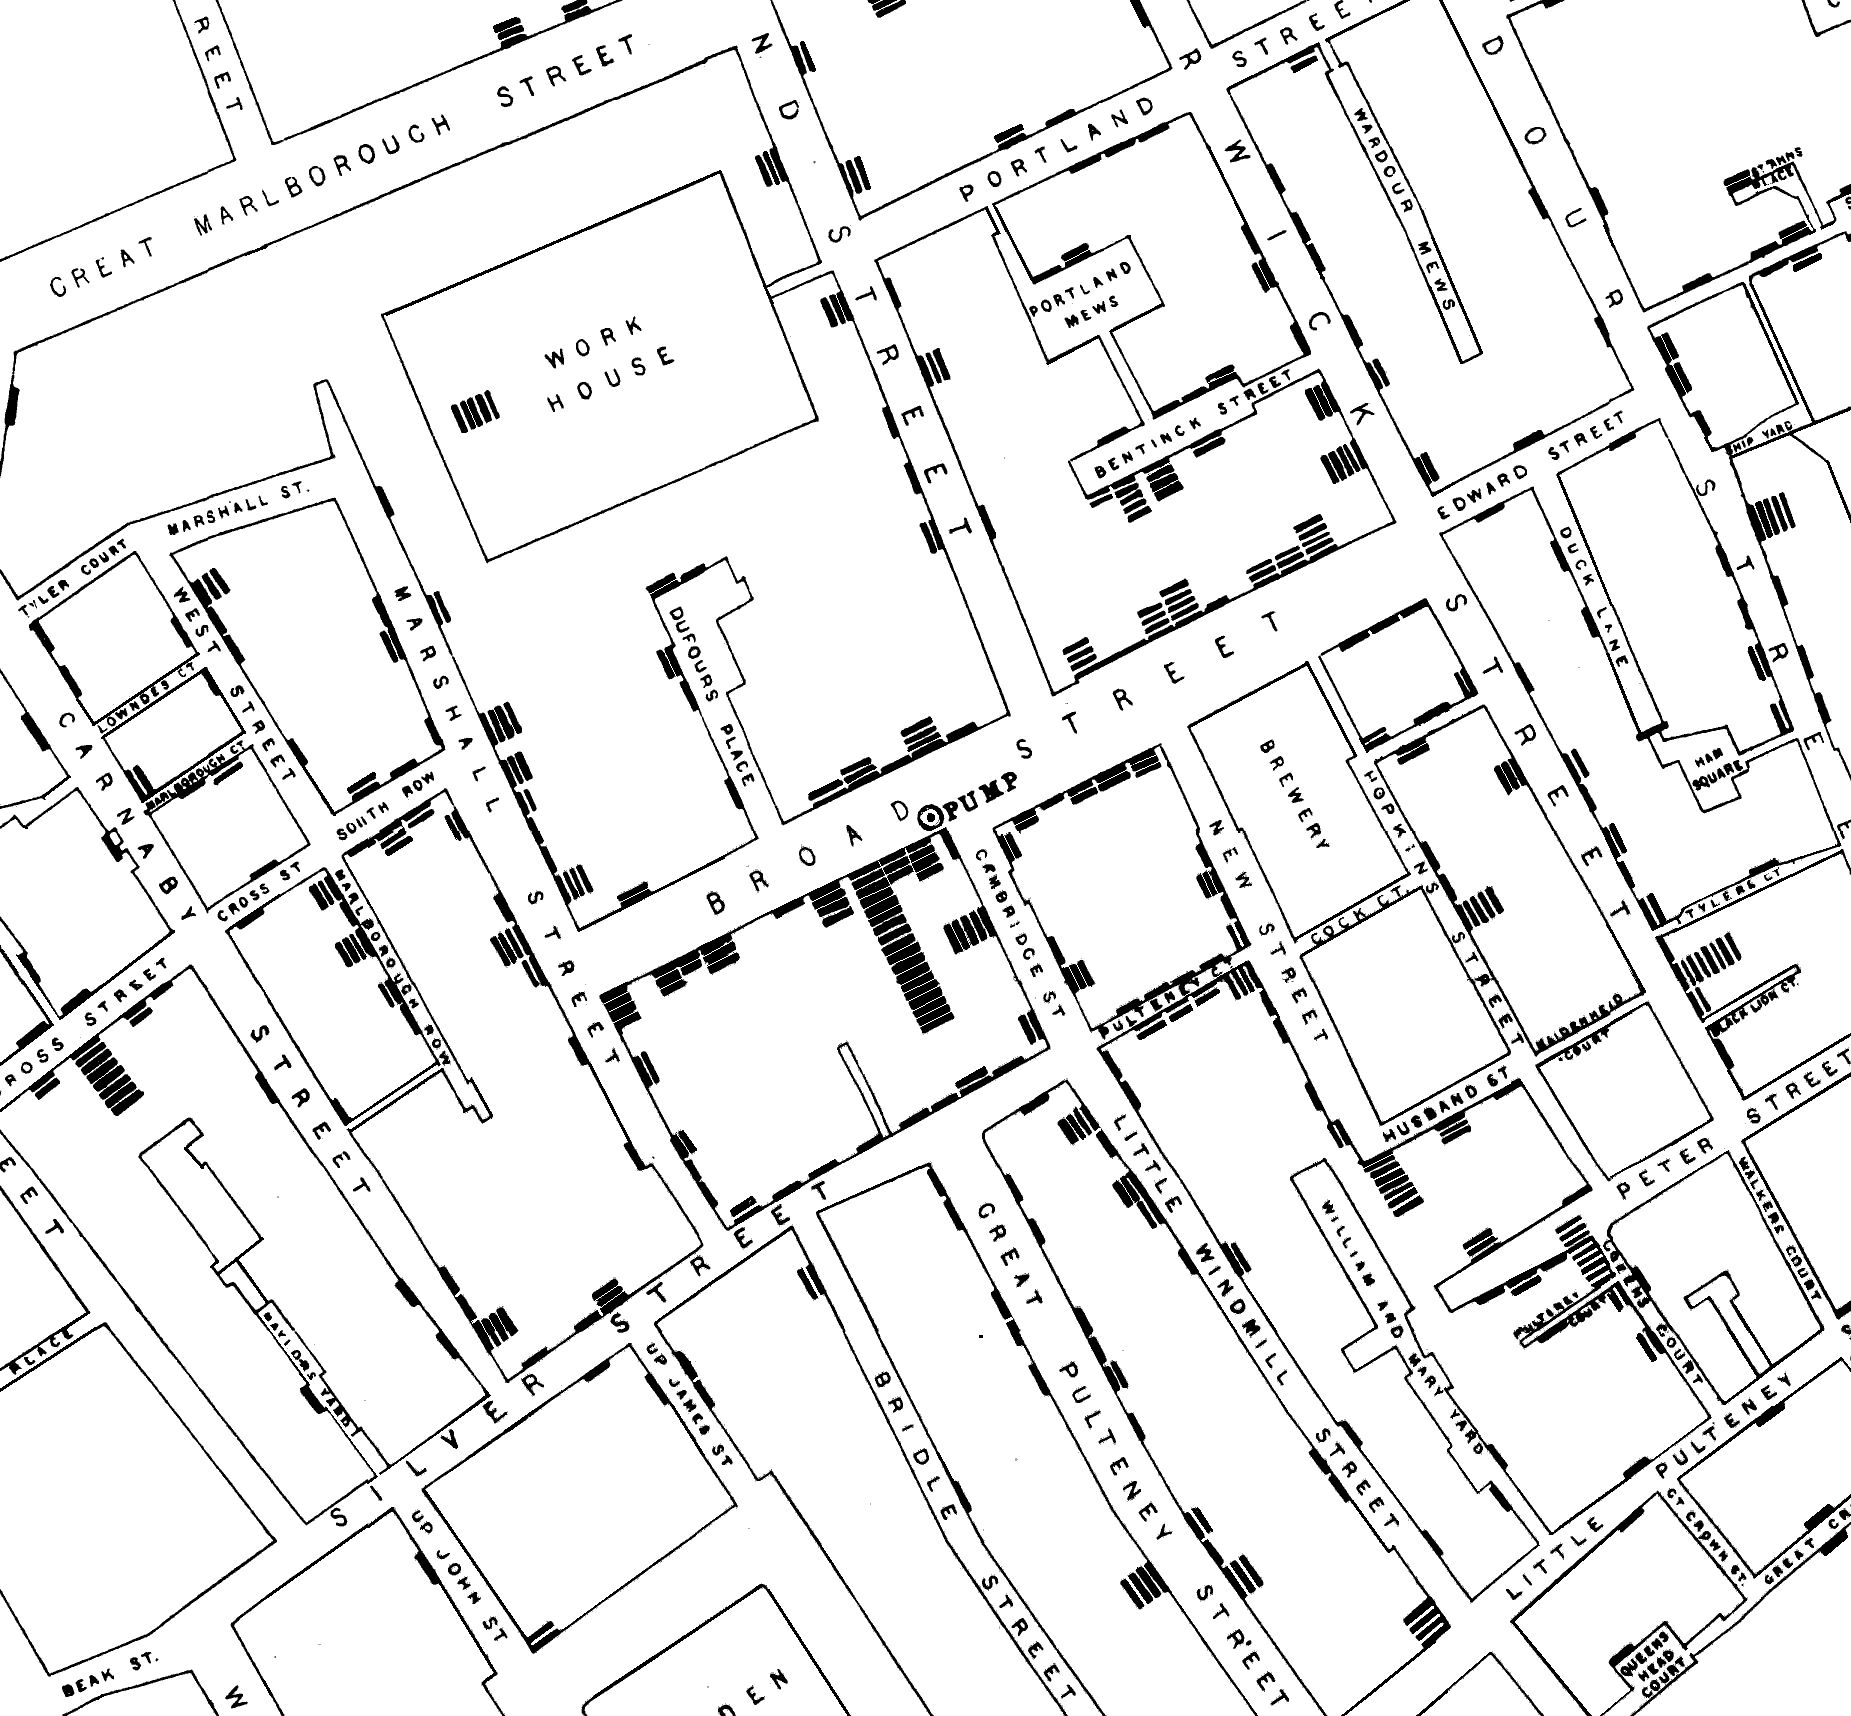
\includegraphics[width=\textwidth]{chap1/snow_map}  
  \caption{John Snow's map is small and marginal.}
  \label{fig:spin_margin}
\end{marginfigure}
